\chapter{Results}
\label{chapter:results}
This chapter states the results of the proposed methods.

\medskip In Section \ref{sec:model_comparison}, we show the results of the trained models on different stages of the dataset.

\medskip Section \ref{sec:model_improvements_results} contains results of improvements of the training pipeline proposed in Section \ref{sec:general_changes}.

\medskip In Section \ref{sec:model_inspection_results}, we depict how different backbones' sizes and weight decay affected the model's performance.

\medskip Section \ref{sec:ensembling_results} reports the influence of ensembling of neural networks. Note that in this section, we obtain the best-performing model.

\medskip Section \ref{sec:dental_restoration_results} contains results of algorithms for segmentation of dental restorations.

\medskip In Section \ref{sec:result_comparision_with_lit}, we compare the results of our best-performing model with the literature.

\medskip In the final Section \ref{sec:visualization} of this chapter, we show figures to showcase the performance of our models.

\section{Model comparison on different datasets}
\label{sec:model_comparison}
This section compares the performance of different model architectures and their backbones. It is divided into five subsections corresponding to five stages of the dataset. For more details about the dataset, see Section \ref{sec:dataset:dental_caries}. For each of the five stages of the dataset, we report the average precision metric on the test part of the dataset. The training of all models was conducted according to the training protocol described in Section \ref{sec:caries_detection}. Tables in this section use abbreviation described in Section \ref{sec:methods:nns}.

\subsection{Stage one dataset}
In Table \ref{tab:model_results:stage_one} the reader can see results obtained on the first stage of the dataset. None of the trained models performed well, especially the Faster R-CNN model achieved low average precision values. We attribute that to the inhomogeneity of the dataset (as described in Section \ref{sec:dataset:second_stage}) and to the low amount of data.
\begin{table}[H]
    \centering
    \begin{tabular}{|l|c|c|c|c|c|c|}
        \hline
        Model           & $AP$  & $AP@.5$ & $AP@.75$ & $AP@.5_S$ & $AP@.5_M$ & $AP@.5_L$ \\ \hline
        FRCNN-R50       & 0.045 & 0.168   & 0.0064   & 0.109     & 0.187     & 0.141     \\ \hline
        YOLOv3          & 0.078 & 0.238   & -        & -         & -         & -         \\ \hline
        YOLOv5-l6       & 0.082 & 0.258   & 0.02     & 0.211     & 0.309     & 0.327     \\ \hline
        YOLOv5-x6       & 0.087 & 0.268   & 0.04     & 0.204     & 0.324     & 0.302     \\ \hline
        EfficientDet-D4 & 0.081 & 0.242   & 0.007    & 0.198     & 0.234     & 0.287     \\ \hline
    \end{tabular}
    \caption{Comparison of the trained models on the stage one dataset}
    \label{tab:model_results:stage_one}
\end{table}

\subsection{Stage two dataset}
Even though the dataset grew in size by more than 50\% since stage one, from Tables \ref{tab:model_results:stage_one} and \ref{tab:model_results:stage_two}, we see that the YOLOv3 model improved by less than $10\%$ . On the contrary, the performance of YOLOv5 model improved by circa $25\%$. Due to the low performance of YOLOv3 and its similarity with superior YOLOv5 architecture, we will not experiment with YOLOv3 in the following sections.
In the last two rows of Table \ref{tab:model_results:stage_two}, we can see the discrepancy in the average precision when evaluated on the test and train part of the dataset. This ensures us that the model can fit the data well, and we only need to alleviate the generalization gap.
\begin{table}[H]
    \centering
    \begin{tabular}{|l|c|c|c|c|c|c|}
        \hline
        Model            & $AP$  & $AP@.5$ & $AP@.75$ & $AP@.5_S$ & $AP@.5_M$ & $AP@.5_L$ \\ \hline
        YOLOv3           & 0.093 & 0.258   & -        & -         & -         & -         \\ \hline
        YOLOv5-l6        & 0.097 & 0.318   & 0.03     & 0.281     & 0.310     & 0.378     \\ \hline
        YOLOv5-x6        & 0.105 & 0.337   & 0.05     & 0.278     & 0.323     & 0.392     \\ \hline
        EffDet-D4        & 0.089 & 0.296   & 0.01     & 0.272     & 0.291     & 0.342     \\ \hline
        EffDet-D4, train & 0.421 & 0.839   & 0.362    & 0.758     & 0.852     & 0.801     \\ \hline
    \end{tabular}
    \caption{Comparison of the trained model on the stage two dataset}
    \label{tab:model_results:stage_two}
\end{table}

\subsection{Stage three dataset}
As mentioned in Section \ref{sec:dataset:third_stage}, there were no additional data added in this stage, but MDDr. Tichý did a review of the dataset as well as corrected any erroneous annotations. The dataset review increased the $AP@.5$ of the EfficiendDet-D4 model by $76\%$, as can be seen in Tables \ref{tab:model_results:stage_three:test} and \ref{tab:model_results:stage_two}. This significant performance gain suggests that the low performance of models in Tables \ref{tab:model_results:stage_one} and \ref{tab:model_results:stage_two} was caused by errors in the dataset.

Performance of EfficentDet and YOLOv5 models evaluated on training part of dataset can be found in Table \ref{tab:model_results:stage_three:train}.

\begin{table}[H]
    \centering
    \begin{tabular}{|l|c|c|c|c|c|c|c|}
        \hline
        Model     & $AP$  & $AP@.3$ & $AP@.5$ & $AP@.75$ & $AP@.5_S$ & $AP@.5_M$ & $AP@.5_L$ \\ \hline
        YOLOv5-l  & 0.249 & 0.734   & 0.631   & 0.132    & 0.598     & 0.671     & 0.607     \\ \hline
        EffDet-D4 & 0.168 & 0.666   & 0.525   & 0.041    & 0.435     & 0.606     & 0.527     \\ \hline
    \end{tabular}
    \caption{Comparison of trained models on the test part of stage three dataset}
    \label{tab:model_results:stage_three:test}
\end{table}

\subsection{Stage four dataset}
The average precision of models trained on this dataset stage is in Table \ref{tab:model_results:stage_four}. Furthermore, precision-recall values for confidence threshold maximizing F1 score are in Table \ref{tab:model_prf:stage_four}, which is located in Appendix. Even though we introduced multiple new architectures and revisited Faster R-CNN with two different backbones, the performance gain obtained in this stage was not as prominent as the one observed when moving from stage three to stage four.

In Table \ref{tab:model_results:stage_four}, we can observe how different architectures differ in their performance on small, medium-sized, and large boxes. Comparing YOLOv5-m6 and RetinaNet-ResNet50 models shows that their overall performance (measured by $AP@.5$) almost matches, but when comparing their $AP@.5_L$ metrics, we see a $15\%$ difference. We try to exploit this behavior by the approach described in Section \ref{sec:methods_area_aware_ens}.

\begin{table}[H]
    \begin{tabular}{|c|c|c|c|c|c|c|}
        \hline
        Model      & $AP$  & $AP@.5$ & $AP@.75$ & $AP@.5_S$ & $AP@.5_M$ & $AP@.5_L$ \\ \hline
        FRCNN-R101 & 0.285 & 0.675   & 0.198    & 0.568     & 0.717     & 0.772     \\ \hline
        FRCNN-R50  & 0.284 & 0.658   & 0.204    & 0.557     & 0.695     & 0.77      \\ \hline
        YOLOv5-m6  & 0.288 & 0.644   & 0.209    & 0.593     & 0.667     & 0.766     \\ \hline
        YOLOv5-l6  & 0.284 & 0.644   & 0.203    & 0.551     & 0.701     & 0.612     \\ \hline
        EffDet-D4  & 0.251 & 0.605   & 0.15     & 0.49      & 0.677     & 0.545     \\ \hline
        RetN-swint & 0.266 & 0.66    & 0.175    & 0.497     & 0.721     & 0.786     \\ \hline
        RetN-R50   & 0.263 & 0.643   & 0.174    & 0.547     & 0.696     & 0.663     \\ \hline
    \end{tabular}
    \caption{Performance comparison of multiple models trained on the stage four dataset}
    \label{tab:model_results:stage_four}
\end{table}

\subsection{Stage five}
The results in Table \ref{tab:model_results:stage_five} show a steady improvement compared to those in Table \ref{tab:model_results:stage_four}. We see that YOLOv5-l6 achieved worse results than in stage four. This result is not emphasized since we believe that if trained multiple times, the results of this architecture would eventually improve. On the contrary, we observe that the EfficientDet-D4 model lagged behind YOLOv5 in all stages of the dataset. Therefore, in Section \ref{sec:methods:group_norm} we experiment with usage of group normalization.
\begin{table}[H]
    \begin{tabular}{|c|c|c|c|c|c|c|c|}
        \hline
        Model      & $AP$  & $AP@.5$ & $AP@.75$ & $AP@.5_S$ & $AP@.5_M$ & $AP@.5_L$ \\ \hline
        FRCNN-R101 & 0.328 & 0.71    & 0.263    & 0.613     & 0.742     & 0.816     \\ \hline
        FRCNN-R50  & 0.334 & 0.715   & 0.273    & 0.595     & 0.757     & 0.809     \\ \hline
        YOLOv5-m6  & 0.346 & 0.708   & 0.284    & 0.622     & 0.744     & 0.754     \\ \hline
        YOLOv5-l6  & 0.295 & 0.625   & 0.232    & 0.533     & 0.691     & 0.489     \\ \hline
        EffDet-D4  & 0.288 & 0.648   & 0.219    & 0.548     & 0.699     & 0.655     \\ \hline
        RetN-swint & 0.328 & 0.72    & 0.241    & 0.565     & 0.776     & 0.775     \\ \hline
    \end{tabular}
    \caption{Performance comparison of multiple models based on mean average precision metrics}
    \label{tab:model_results:stage_five}
\end{table}

\section{Improvements}
\label{sec:model_improvements_results}
\subsection{Training protocol improvements}
The average precision of models trained with incorporated improvements proposed in Section \ref{sec:general_changes}, can be seen in Table \ref{tab:improved:precision}. Furthermore, average recall values can be observed in Table \ref{tab:improved:recall}, which is located in the Appendix, together with a table of precision-recall values for a given confidence threshold\ref{tab:imrpoved:prf}.

Even though the best performing model in Table \ref{tab:improved:precision} improved negligibly over the best performing one in Table \ref{tab:model_results:stage_five}. We notice that models achieved better results on average along with more stable training. In this stage, we newly used YOLOv5-s and EfficienDet-D1. Despite both being low-parameter networks, they performed almost on par with others.
\begin{table}[H]
    \centering
    \begin{tabular}{|c|c|c|c|c|c|c|c|}
        \hline
        Model      & $AP$  & $AP@.3$ & $AP@.5$ & $AP@.75$ & $AP@.5_S$ & $AP@.5_M$ & $AP@.5_L$ \\ \hline
        YOLOv5-l6  & 0.347 & 0.796   & 0.725   & 0.291    & 0.597     & 0.772     & 0.753     \\ \hline
        YOLOv5-m6  & 0.343 & 0.795   & 0.719   & 0.287    & 0.636     & 0.752     & 0.785     \\ \hline
        YOLOv5-s6  & 0.327 & 0.79    & 0.697   & 0.281    & 0.559     & 0.739     & 0.826     \\ \hline
        Effdet-D1  & 0.319 & 0.787   & 0.701   & 0.251    & 0.584     & 0.752     & 0.808     \\ \hline
        FRCNN-R50  & 0.311 & 0.788   & 0.705   & 0.231    & 0.629     & 0.737     & 0.788     \\ \hline
        FRCNN-R101 & 0.316 & 0.792   & 0.688   & 0.239    & 0.563     & 0.732     & 0.793     \\ \hline
        RetN-swint & 0.325 & 0.803   & 0.723   & 0.249    & 0.579     & 0.78      & 0.758     \\ \hline
    \end{tabular}
    \caption{Comparison of AP values between different models trained by an improved training protocol}
    \label{tab:improved:precision}
\end{table}



\subsection{Group normalization}
\label{sec:group_nromalization:res}
Chart of $AP@.5$ for EfficientDet-D4 models with batch-normalization layers and group normalization layers can be found in Figure \ref{fig:batch_group_diff}. Model using batch normalization achieved $AP@.5$ of 0.634 on the test dataset, outperforming the model using group normalization with $AP@.5=0.694$. Despite the performance increase induced by group normalization, the EfficientDet-D4 model performed comparably with the models in Table \ref{tab:improved:precision}. Therefore, we stopped using this model further on, because the training of this model was also more computationally demanding than the rest of the models.
\begin{figure}[H]
    \centering
    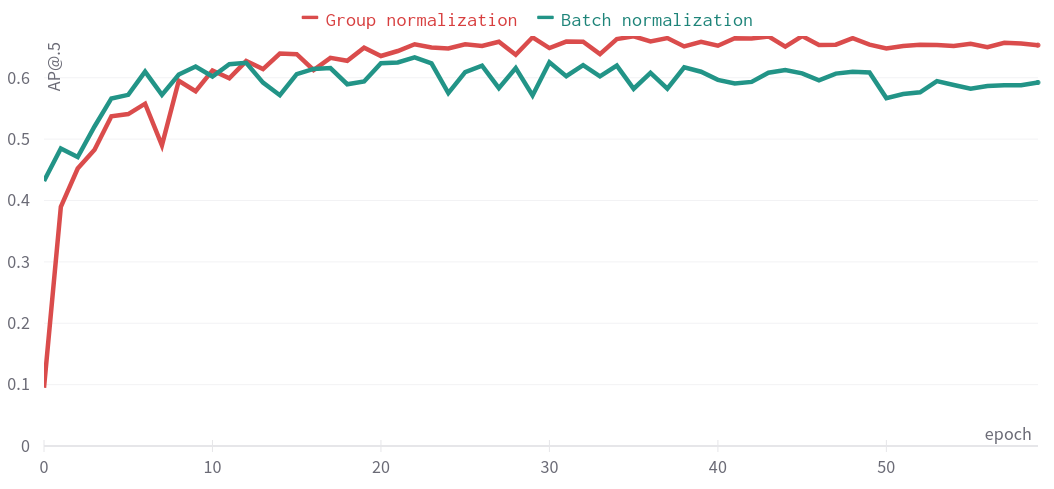
\includegraphics[width=0.9\textwidth]{images/group_norm_batch_norm.png}
    \caption{Difference in $AP@.5$ amog EfficientDet-D4 model with batch normalization and group normalization}
    \label{fig:batch_group_diff}
\end{figure}

\section{Model inspection}
\label{sec:model_inspection_results}
\subsection{Size of backbone}
The table \ref{tab:backbone_comparison}was computed from the statistics of 29 models, where each type of backbone was represented by 8 to 12 models. The columns mean, std, max and min denote statistics of $AP@.5$ obtained by trained models on the test set. Furthermore, we can inspect the size of a given backbone, which is induced by its number of parameters (Par) and floating-point operations FLOPs. The last column of Table $\ref{tab:backbone_comparison}$ shows the average time required to train the given backbone for $60$ epochs.
\begin{table}[H]
    \begin{tabular}{|c|c|c|c|c|c|c|c|}
        \hline
        Backbone & Mean  & Std.   & Max   & Min   & Par[M] & FLOPs[G] & Time[h] \\ \hline
        Small    & 0.68  & 0.0197 & 0.651 & 0.697 & 12     & 21       & 2.1     \\ \hline
        Medium   & 0.696 & 0.0126 & 0.669 & 0.719 & 35     & 63       & 3.5     \\ \hline
        Large    & 0.703 & 0.0136 & 0.681 & 0.725 & 76     & 141      & 5.2     \\ \hline
    \end{tabular}
    \caption{Comparison of $AP.@5$ metric for different backbones of YOLOv5 architecture}
    \label{tab:backbone_comparison}
\end{table}

\subsection{Weight decay}
In Figures \ref{fig:fasterrcnn_weight_decay} and \ref{fig:yolo_weight_decay}, we see the comparison of Faster-RCNN and YOLOv5 models using different weight decay. The results obtained by evaluating trained models on the test part of the dataset did not differ across the values of weight decay.
\begin{figure}[H]
    \begin{floatrow}[2]
        \ffigbox[\FBwidth]{
            \caption{$AP@.5$ of Faster-RCNN model with varying weight decay values. The metric is computed on the validation part of the dataset during training.  \label{fig:fasterrcnn_weight_decay}}
        }{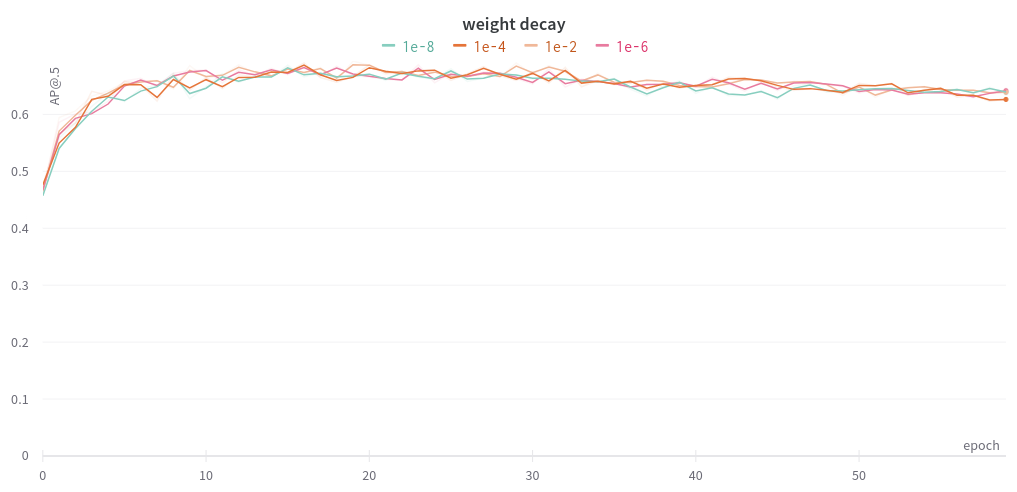
\includegraphics[width=\linewidth]{images/weight_decay_fasterrcnn.png}}
        \ffigbox[\FBwidth]{\caption{$AP@.5$ of YOLOv5 model with varying weight decay values. The metric is computed on the validation part of the dataset during training. \label{fig:yolo_weight_decay}}}
        { 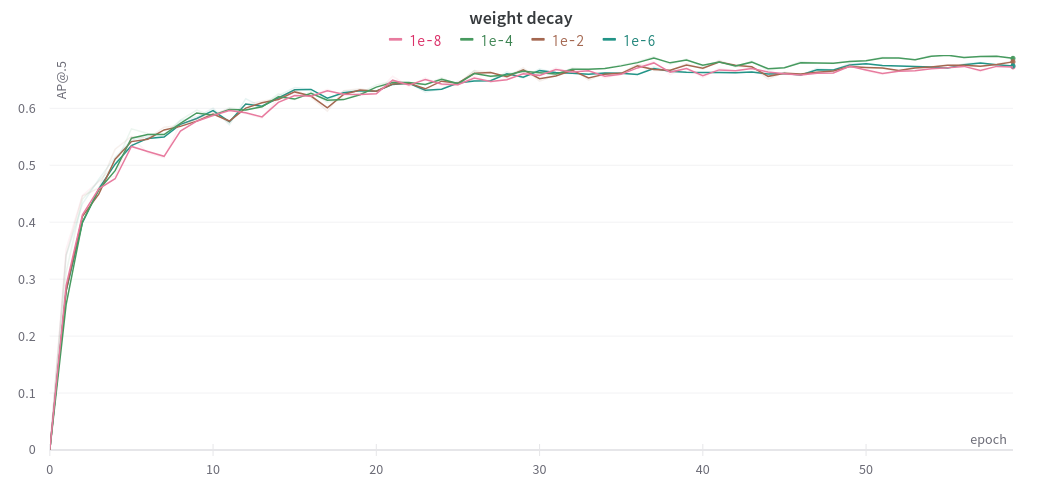
\includegraphics[width=\linewidth]{images/weight_decay_yolo.png} }
    \end{floatrow}
\end{figure}

\section{Ensembling}
\label{sec:ensembling_results}
In this section, we show the performance of model ensemblings with handpicked parameters \ref{subsec:handpicked}as well as ensemblings obtained by parameters found by a grid-search. Furthermore, we report how the diversity of models involved in the ensembling affects its results.
\subsection{Manually-picked parameters}
\label{subsec:handpicked}
In Table \ref{tab:model_ensembling:handpicked}, the reader can see the results obtained by handpicking circa ten sets of hyperparameters based on our qualified guess. We then evaluated the hyperparameters on the validation part of the dataset, and the best-performing ones were selected and evaluated on the test part of the dataset. The first group (G1) contained the following models trained on the stage four dataset: RetinaNet-swint, YOLOv5-m, and RetinaNet-ResNet50. The second group (G2) was composed of Faster R-CNN-Resnet101, YOLOv5-m, and RetinaNet-swint. All of those models were trained on stage four of the dataset. From the Tables \ref{tab:model_ensembling:handpicked} and \ref{tab:model_results:stage_four}, we can infer that ensembling of models improved $AP@.5$ by $3\%$ over the best performing model included in the ensembling.
\begin{table}[H]
    \begin{tabular}{|c|c|c|c|c|c|c|c|}
        \hline
        Models & $AP$  & $AP@.3$ & $AP@.5$ & $AP@.75$ & $AP@.5_S$ & $AP@.5_M$ & $AP@.5_L$ \\ \hline
        G1     & 0.303 & 0.776   & 0.694   & 0.216    & 0.605     & 0.729     & 0.803     \\ \hline
        G2     & 0.305 & 0.783   & 0.695   & 0.218    & 0.598     & 0.733     & 0.807     \\ \hline
    \end{tabular}
    \caption{WBF ensembling of multiple models, where we handpicked the parameters of the ensembling process. The models were trained on the stage four dataset.}
    \label{tab:model_ensembling:handpicked}
\end{table}
\subsection{Grid search results}
\label{subsec:gridsearched}
All models included in the ensembling were trained on the stage-five dataset. Therefore, their results are in Table \ref{tab:model_results:stage_five}.

The best hyperparameters for a given ensembling method found by a grid search are in Table \ref{tab:ensemble_params:grid_search}. We omitted parameter $\sigma$ used only in S-NMS from the table. Its optimal value, according to the grid search, was $0.8$.
The average precision of models ensembled with parameters from Table \ref{tab:ensemble_params:grid_search} is available in Table \ref{tab:precision:grid_search} and average recall values are in Table \ref{tab:recall:grid_search}. Precision and recall values based on the confidence threshold that maximizes F-score can be seen in Table \ref{tab:ensembling_prf:grid_search}. In Tables \ref{tab:ensemble_params:grid_search} and \ref{tab:precision:grid_search}, we used notations introduced in Section \ref{sec:model_ensembling}. By WBF-A, we refer to the method proposed in Section \ref{sec:methods_area_aware_ens}, where S,M,L mean weights for small, medium-sized, and large boxes.

\begin{table}[H]
    \begin{tabular}{|c|c|c|c|c|c|c|}
        \hline
        Method  & FRCNN & YOLOv5 & RetN  & FRCNN & $T$  \\
                & R50   & m6     & swint & R101  &      \\ \hline
        NMS     & 1     & 0.4    & 0.4   & 0.85  & 0.6  \\ \hline
        SNMS    & 1     & 0.12   & 0.12  & 0.12  & 0.7  \\ \hline
        NMW     & 0.85  & 0.25   & 0.70  & 0.85  & 0.45 \\ \hline
        WBF     & 1     & 0.4    & 0.85  & 0.85  & 0.65 \\ \hline
        WBF-A S & 0.94  & 0.31   & 0.98  & 0.72  & 0.64 \\ \hline
        WBF-A M & 0.77  & 0.47   & 0.85  & 0.69  & 0.64 \\ \hline
        WBF-A L & 0.84  & 0.31   & 0.88  & 0.91  & 0.64 \\ \hline
    \end{tabular}
    \caption{Hyperparameter values of ensembling methods found by a grid-search}
    \label{tab:ensemble_params:grid_search}
\end{table}


\begin{table}[H]
    \centering
    \begin{tabular}{|c|c|c|c|c|c|c|c|}
        \hline
        Method & $AP$  & $AP@.3$ & $AP@.5$ & $AP@.75$ & $AP@.5_S$ & $AP@.5_M$ & $AP@.5_L$ \\ \hline
        NMS    & 0.346 & 0.818   & 0.735   & 0.28     & 0.618     & 0.775     & 0.829     \\ \hline
        SNMS   & 0.348 & 0.807   & 0.722   & 0.295    & 0.609     & 0.758     & 0.819     \\ \hline
        NWM    & 0.364 & 0.829   & 0.759   & 0.302    & 0.641     & 0.802     & 0.854     \\ \hline
        WBF    & 0.378 & 0.832   & 0.77    & 0.323    & 0.663     & 0.807     & 0.875     \\ \hline
        WBF-A  & 0.376 & 0.832   & 0.768   & 0.318    & 0.651     & 0.806     & 0.875     \\ \hline
    \end{tabular}
    \caption{Average precision of models ensembled with parameters from Table \ref{tab:ensemble_params:grid_search}}
    \label{tab:precision:grid_search}
\end{table}


\subsection{Assessing the importance of different models}
\label{sec:results:improtance_of_models}
In this section, we present ensembling results based on the approach from Section \ref{sec:methods:assesing_importance}. In Tables \ref{tab:precision:ensemble_compare}, \ref{tab:recall:ensemble_compare} and \ref{tab:ensembling_prf:ensemble compare}, we see results of ensembles composed of different models. Note that the ensembling of varying architectures (Mixture) achieved the best results out of all models evaluated in this thesis. We will use this model to compare our results with related publications.

From Table \ref{tab:precision:ensemble_compare}, we can see that the usage of varying backbones increases the gain in average precision by circa $1.5\%$, when compared to the ensembling with the identical backbones. Furthermore, using different architectures increased the performance by an additional $3.2\%$. Please note that models included in ensembling with different architectures had an average $AP@.5$ by $2\%$  higher than models included in the former two ensembling approaches, see Table \ref{tab:ensemble_models_involved}. If we adjust the results for that, we expect a $1.2\%$ gain solely from using models with varying architecture.


The importance of individual models in the ensembling is in Figure \ref{fig:ensembling_parameters_importance} for Mixture architectures and in Figures \ref{fig:ensembling_hparams_imprtance_yolo_m}, \ref{fig:ensembling_hparams_imprtance_yolo_mix} located in Appendix for the remaining two groups of models.


\begin{table}[h]
    \centering
    \begin{tabular}{|c|c|c|c|c|c|c|c|}
        \hline
        Models  & $AP$  & $AP@.3$ & $AP@.5$ & $AP@.75$ & $AP@.5_S$ & $AP@.5_M$ & $AP@.5_L$ \\ \hline
        Mixture & 0.389 & 0.838   & 0.774   & 0.338    & 0.665     & 0.811     & 0.876     \\ \hline
        Y5-mix  & 0.379 & 0.819   & 0.75    & 0.34     & 0.636     & 0.79      & 0.84      \\ \hline
        Y5-m    & 0.368 & 0.812   & 0.741   & 0.329    & 0.648     & 0.775     & 0.844     \\ \hline
    \end{tabular}
    \caption{Average precision of ensemble models}
    \label{tab:precision:ensemble_compare}
\end{table}


\begin{table}[h]
    \centering
    \begin{tabular}{|c|c|c|c|c|c|c|c|}
        \hline
        Models  & $AR$  & $AR@.5_{10}$ & $AR@.5$ & $AR@.75$ & $AR@.5_S$ & $AR@.5_M$ & $AR@.5_L$ \\ \hline
        Mixture & 0.586 & 0.917        & 0.978   & 0.582    & 0.946     & 0.991     & 0.991     \\ \hline
        Y5-mix  & 0.579 & 0.911        & 0.959   & 0.599    & 0.929     & 0.972     & 0.972     \\ \hline
        Y5-m    & 0.562 & 0.906        & 0.949   & 0.572    & 0.909     & 0.964     & 0.964     \\ \hline
    \end{tabular}
    \caption{Average recall of models ensembled by parameters from Table \ref{tab:ensemble_params:grid_search}}
    \label{tab:recall:ensemble_compare}
\end{table}


\begin{table}[h]
    \begin{tabular}{|c|c|c|c|c|}
        \hline
        Models     & Precision & Recall & F-score & Confidence threshold \\ \hline
        Mixture    & 0.751     & 0.7    & 0.725   & 0.294                \\ \hline
        YOLOv5-mix & 0.728     & 0.69   & 0.708   & 0.241                \\ \hline
        YOLOv5-m   & 0.726     & 0.67   & 0.697   & 0.272                \\ \hline
    \end{tabular}
    \caption{Precision, recall, and F-score based on the confidence threshold for different ensembling methods}
    \label{tab:ensembling_prf:ensemble compare}
\end{table}

\begin{figure}
    \centering
    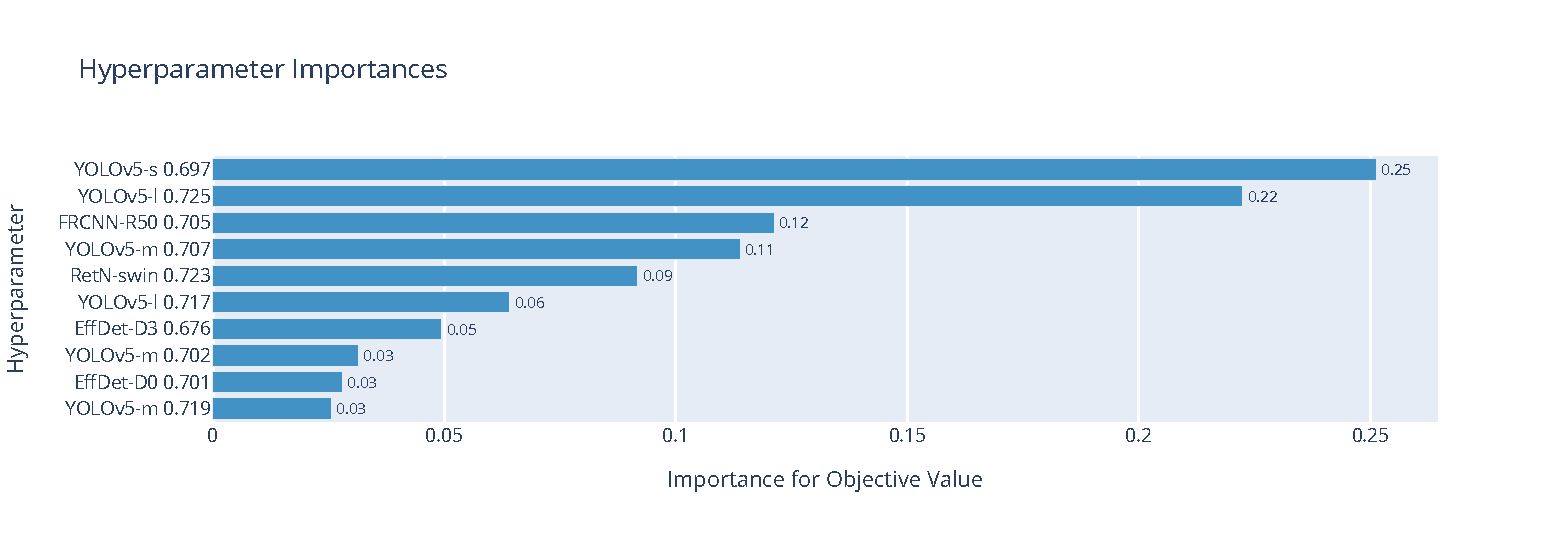
\includegraphics[width=\linewidth]{images/ensemble_all_importance.pdf}
    \caption{Importance of different models during ensembling with different architectures}
    \label{fig:ensembling_parameters_importance}
\end{figure}


\section{Dental restorations segmentation}
In the following section, we report results obtained by a non-deep learning pipeline for dental restorations segmentation proposed in Section \ref{sec:methods:seg_nondl}, as well as deep learning model U-Net trained according to the description in Section \ref{sec:methods:seg_unet}.
\label{sec:dental_restoration_results}
\subsection{Non-deep learning approach}
Hyperparameters ensuring the best performance on the validation part of the dataset are in Table \ref{tab:nondl_restorations:best_params}. The performance of the pipeline given the parameters in Table \ref{tab:nondl_restorations:best_params} on the test dataset can be seen in Table \ref{tab:nondl_results}. The segmentation of the image together with output after each auxiliary stage is in Figure \ref{fig:segmentation_sample_nondl}.

\begin{figure}[h]
    \centering
    \begin{subfigure}[b]{\textwidth}
        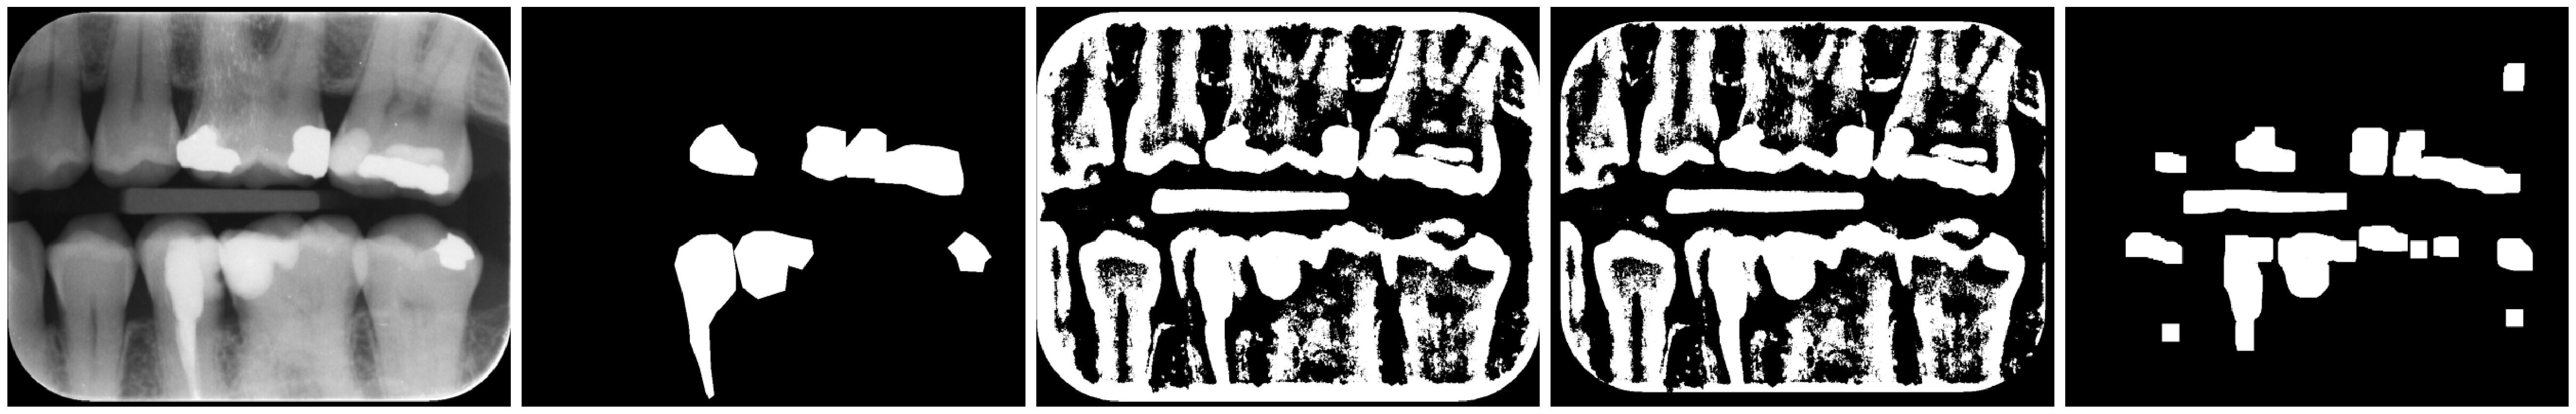
\includegraphics[width=1\linewidth]{images/segmentation_nondl_gauss_12.pdf}
        \caption{Gaussian adaptive thresholding}
    \end{subfigure}

    \begin{subfigure}[b]{\textwidth}
        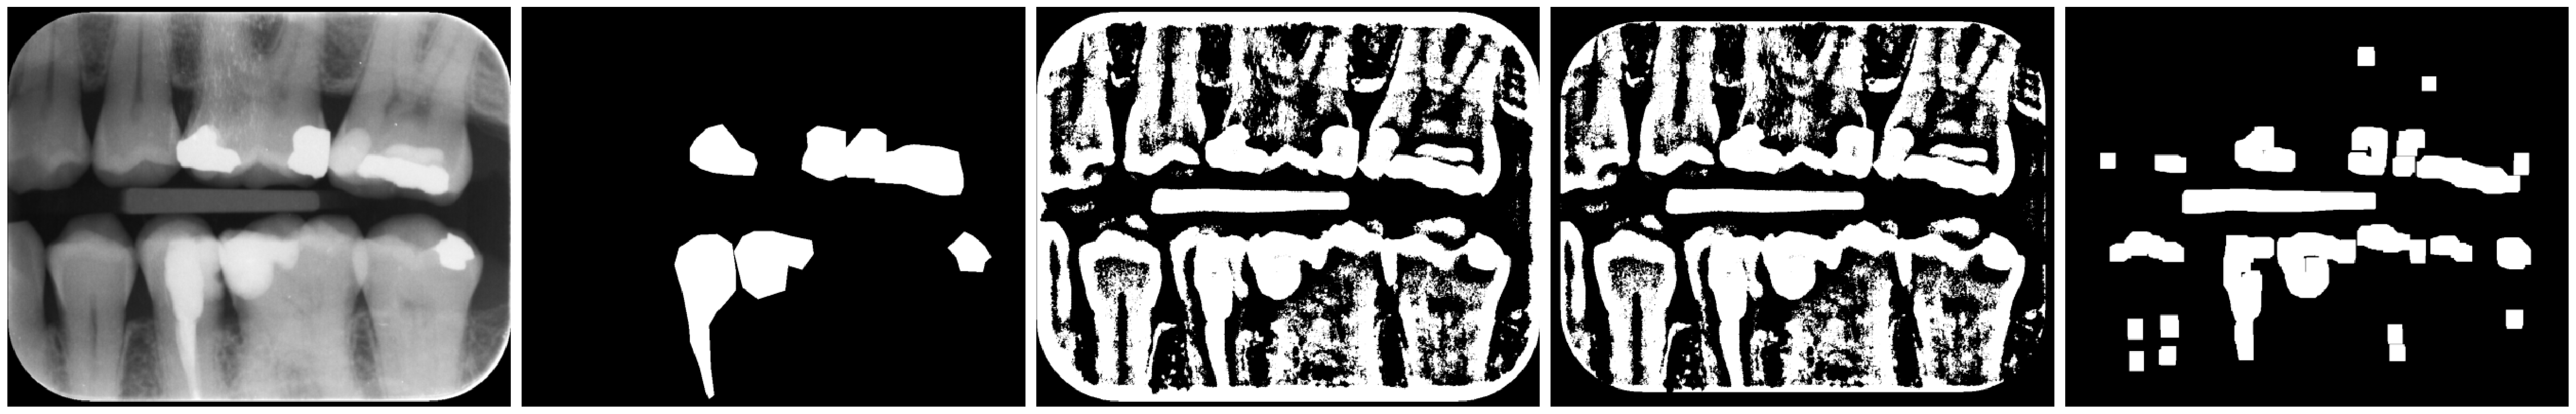
\includegraphics[width=1\linewidth]{images/segmentation_nondl_mean_12.pdf}
        \caption{Mean adaptive thresholding}
    \end{subfigure}
    \caption{From the left: X-ray image, ground-truth pixel mask, thresholded image, removal of border pixels, morphological opening}
    \label{fig:segmentation_sample_nondl}
\end{figure}

\begin{table}[H]
    \begin{tabular}{|c|c|c|c|}
        \hline
        Hyper-parameter & Adaptive mean & Adaptive Gaussian & Otsu's \\ \hline
        $K_t$           & 71            & 83                & -      \\ \hline
        $T$             & 3             & 3                 & -      \\ \hline
        $K_d$           & 41            & 41                & 61     \\ \hline
        $K_o$           & 31            & 36                & 36     \\ \hline
        $K_b$           & -             & -                 & 21     \\ \hline
    \end{tabular}
    \caption{Best hyper-parameters for non-deep learning pipeline}
    \label{tab:nondl_restorations:best_params}
\end{table}


\begin{table}[H]
    \centering
    \begin{tabular}{|c|c|c|}
        \hline
        Model               & Dice  & IOU   \\ \hline
        Adaptive mean       & 0.364 & 0.314 \\ \hline
        Adaptive Gaussian   & 0.328 & 0.274 \\ \hline
        Otus's thresholding & 0.102 & 0.088 \\ \hline
    \end{tabular}
    \caption{Results of non-deep learning approach to dental restorations segmentation given the hyperparameters in Table \ref{tab:nondl_restorations:best_params}}
    \label{tab:nondl_results}
\end{table}



\subsection{U-Net}
Two U-Net models were trained with the settings proposed in Section \ref{sec:methods:seg_unet}. We will call them U-Net-baseline (U-Net-B) and U-Net-improved (U-Net-I). With the letters PP, we denote that the model's output was post-processed by the approach described in Section \ref{sec:segmentation_post_processing}.
In Figure \ref{fig:segmentation_losses}, we see IOU evaluated on the validation dataset throughout the model training, where each line corresponds to a different loss function. We notice that a combination of BCE and soft-Dice loss achieved the highest IOU results, while soft-Dice loss diverged after a promising performance at the beginning of the training.

The best hyperparameters for post-processing of both models are in Table \ref{tab:unet_seg_hyperparams}. In Figure \ref{fig:heatmap_postprocess}, we observe how the choice of different hyperparameters for the post-processing pipeline affected the performance of U-Net-B model.

Figure \ref{fig:segmentation_unet_sample} shows the segmentation results and compares those with the ground truth mask.

\begin{figure}[h]
    \centering
    \begin{subfigure}[b]{\textwidth}
        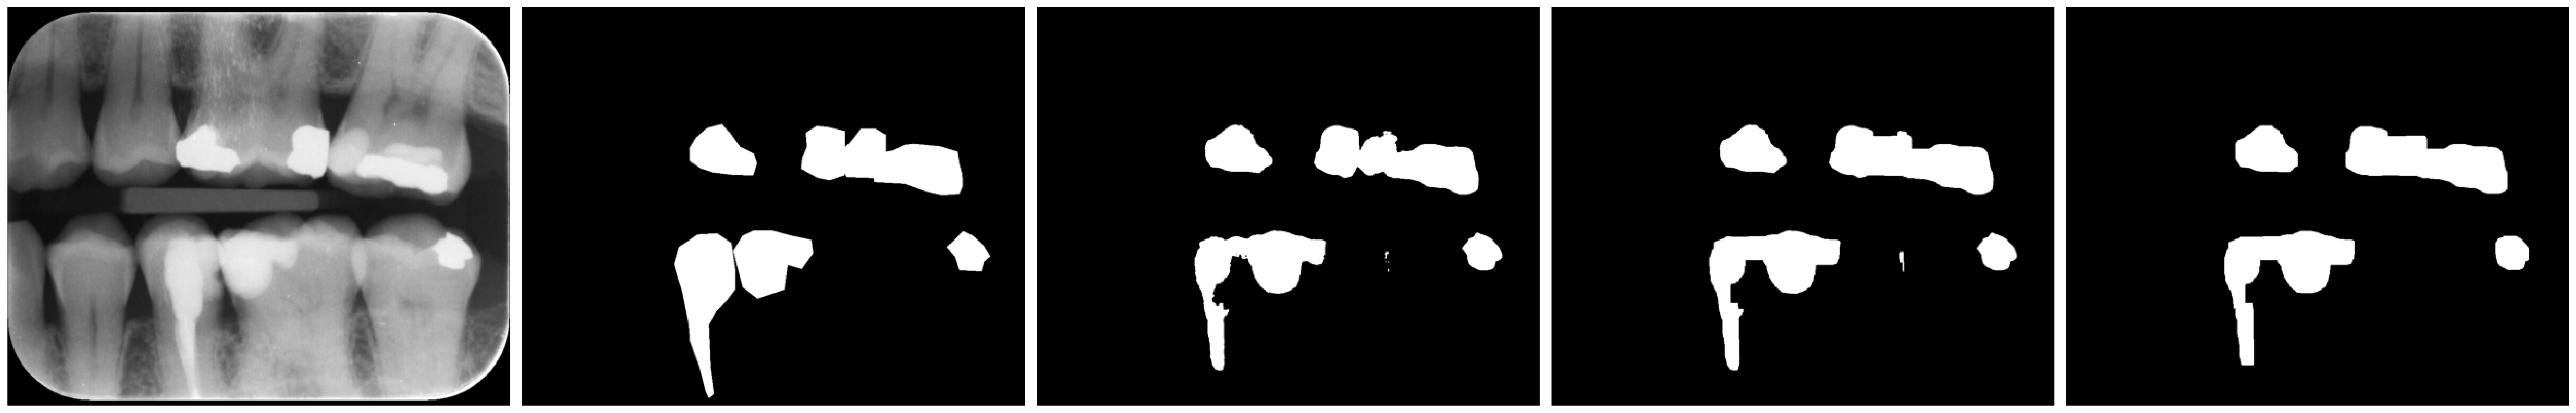
\includegraphics[width=1\linewidth]{images/unet_1_img_12.pdf}
        \caption{Baseline U-Net model}
    \end{subfigure}

    \begin{subfigure}[b]{\textwidth}
        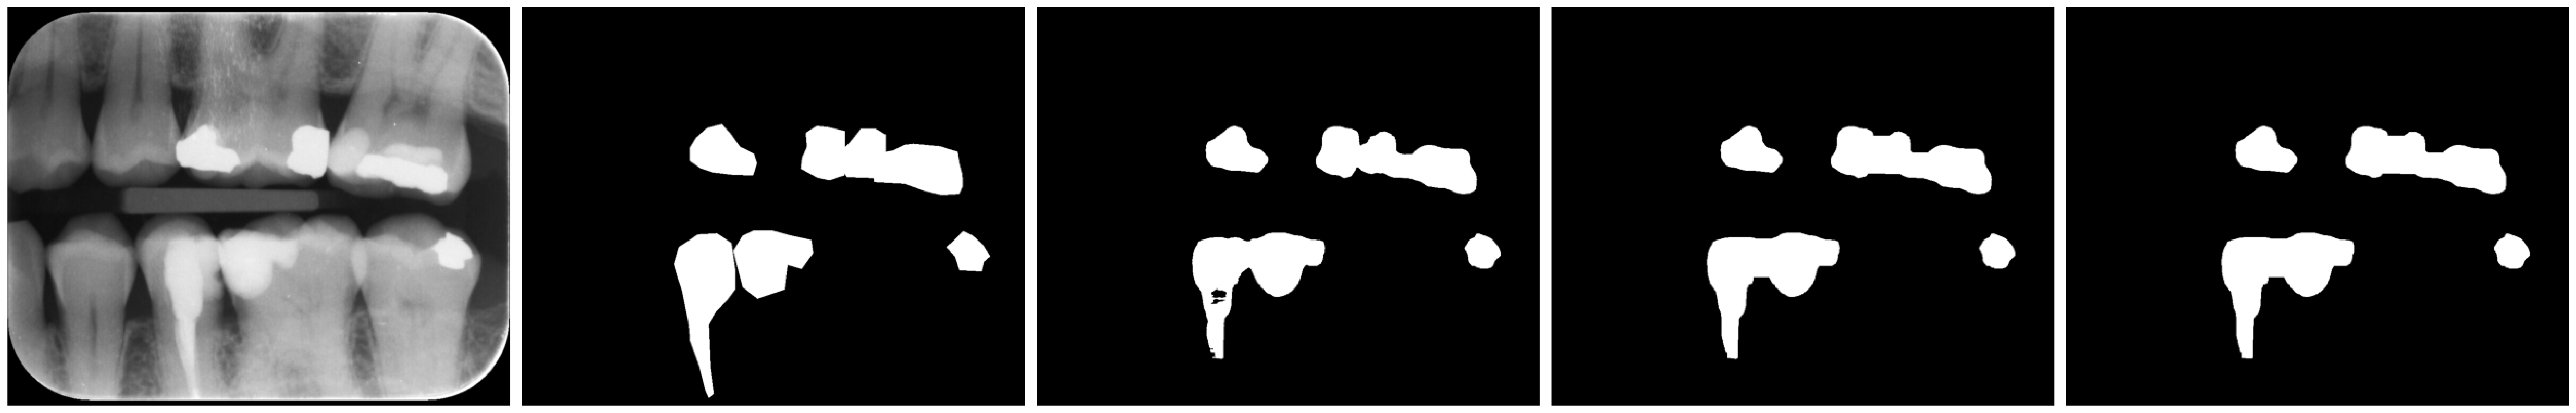
\includegraphics[width=1\linewidth]{images/unet_2_img_12.pdf}
        \caption{Improved U-Net model}
    \end{subfigure}
    \caption{From the left: X-ray image, ground-truth pixel mask, the output of the model, output processed by morphological opening, output post-processed by morphological opening and closing.}
    \label{fig:segmentation_unet_sample}
\end{figure}
\begin{figure}
    \centering
    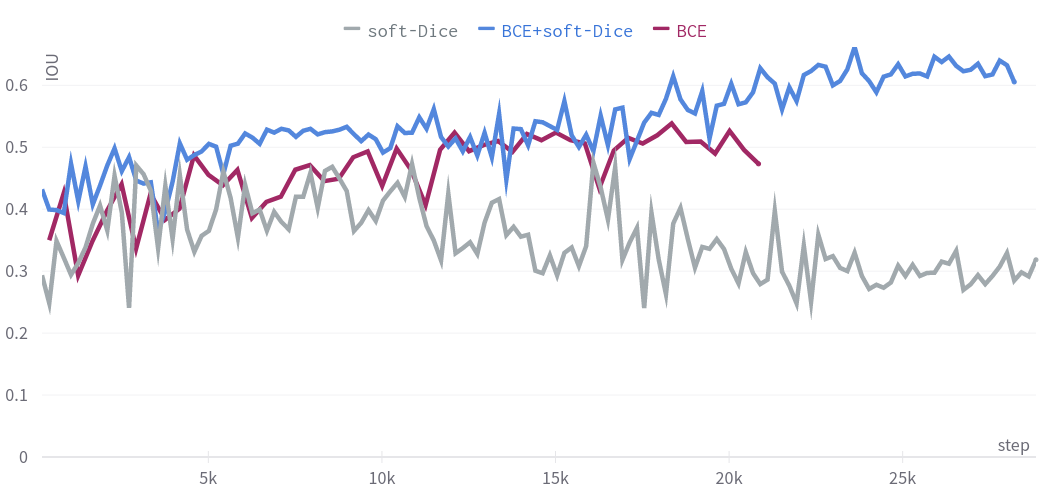
\includegraphics[width=0.8\linewidth]{images/segmentation_losses.png}
    \caption{IOU throughout the training of U-Net model for different loss functions}
    \label{fig:segmentation_losses}
\end{figure}

\begin{figure}[H]
    \centering
    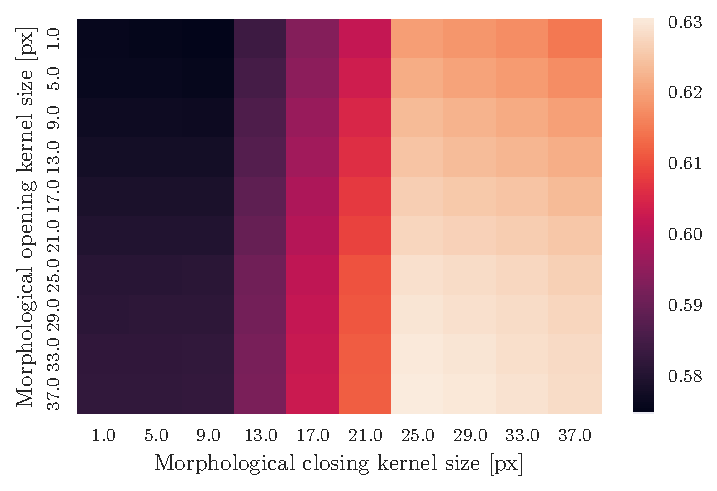
\includegraphics[]{images/heatmap_of_unetpostproc_search.pdf}
    \caption{Value of IOU metric based on the size of kernels $K_o$, $K_c$ in morphological operations that were used for post-processing}
    \label{fig:heatmap_postprocess}
\end{figure}

\begin{minipage}{\textwidth}

    \begin{minipage}[t]{0.48\textwidth}
        \centering
        \makeatletter\def\@captype{table}
        \begin{tabular}{|c|c|c|}
            \hline
            Parameter & $K_o$ & $K_c$ \\ \hline
            U-Net     & 37    & 25    \\ \hline
            U-Net-I   & 33    & 5     \\ \hline
        \end{tabular}
        \caption{Optimal parameters for model post-processing found by a grid-search}
        \label{tab:unet_seg_hyperparams}
    \end{minipage}
    \begin{minipage}[t]{0.48\textwidth}
        \centering
        \makeatletter\def\@captype{table}
        \begin{tabular}{|c|c|c|}
            \hline
            Model      & Dice  & IOU   \\ \hline
            U-Net-B    & 0.663 & 0.575 \\ \hline
            U-Net-B-PP & 0.714 & 0.623 \\ \hline
            U-Net-I    & 0.747 & 0.662 \\ \hline
            U-Net-I-PP & 0.760 & 0.676 \\ \hline
        \end{tabular}
        \caption{Results of U-Net models}
        \label{tab:unet_seg_results}
    \end{minipage}
\end{minipage}


\section{Comparison of results with related publications}
\label{sec:result_comparision_with_lit}
In Table \ref{tab:results_comparison}, we see a comparison of caries detection results of this thesis contrasted to results achieved by related works. We compared with only those who selected a similar approach to ensure at least a minimal amount of comparability.

\begin{table}
    \centering
    \begin{tabular}{|c|c|c|c|c|c|}
        \hline
        Author                                                                 & Precision & Recall & F1-Score & Accuracy & $AP@.5$ \\ \hline
        This thesis                                                            & 0.751     & 0.7    & 0.725    & 0.726    & 0.774   \\ \hline
        Srivastava et al. \cite{Srivastava2017}                                & 0.615     & 0.805  & 0.7      & -        & -       \\ \hline
        Kumar                                   \& Srivastava \cite{Kumar2018} & 0.7       & 0.53   & 0.614    & -        & -       \\ \hline
        Bayrakdar et al. \cite{Bayrakdar2021}                                  & 0.78      & 0.77   & 0.78     & -        & -       \\ \hline
        Bayraktar et al. \cite{Bayraktar2021}                                  & -         & 0.72   & -        & 0.946    & 0.872   \\ \hline
        Cantu et al. \cite{Cantu2020}                                          & -         & 0.75   & 0.73     & 0.8      & -       \\ \hline
    \end{tabular}
    \caption{Comparison of results of this thesis with results in related publications}
    \label{tab:results_comparison}
\end{table}

Note that Cantu et al. \cite{Cantu2020} solved the problem of dental caries localization as a semantic segmentation task. The recall and F1-score are calculated per pixel, while others worked with bounding boxes. However, the reader can still estimate how their work compares to others in table.


\section{Visualization of models}
\label{sec:visualization}
All figures in this section were generated by the best performing ensemble model for caries detection, introduced in Section \ref{tab:precision:ensemble_compare}, and the U-Net-I model (without post-processing).

Figure \ref{fig:recall_fpperimg} shows the relationship between the number of false positives per image and the recall of the model. The graph was truncated and did not include points for $recall > 0.91$ since it would decrease the chart's readability.

Figure \ref{fig:both_models_1} overlays the bitewing image with predictions of both caries detection and restorations segmentation models. For more similar figures, see Appendix \ref{chpater:appendix:preds} and \ref{appendix:model_predictions}



\begin{figure}[h]
    \begin{floatrow}[2]
        \ffigbox[\FBwidth]{
            \caption{Number of false positives per image for a given value of recall \label{fig:recall_fpperimg}}
        }{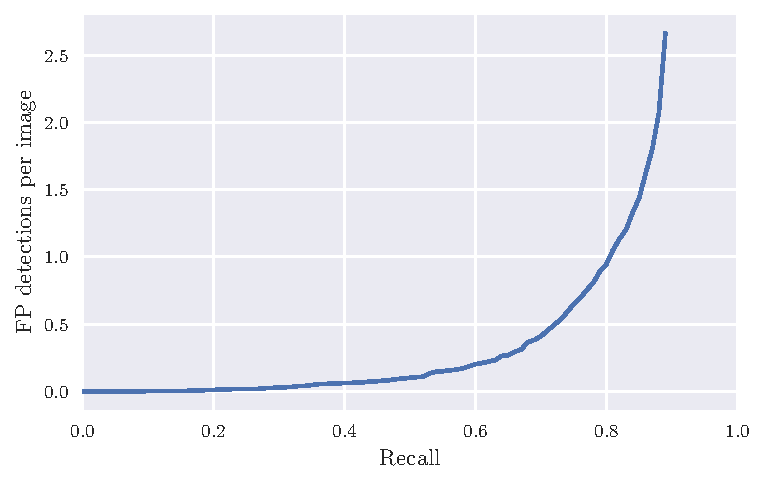
\includegraphics[width=\linewidth]{images/fp_recall.pdf}}
        \ffigbox[\FBwidth]{\caption{Percentage of nondetected dental caries based on the precision of the model \label{fig:precision_nondetected}}}
        { 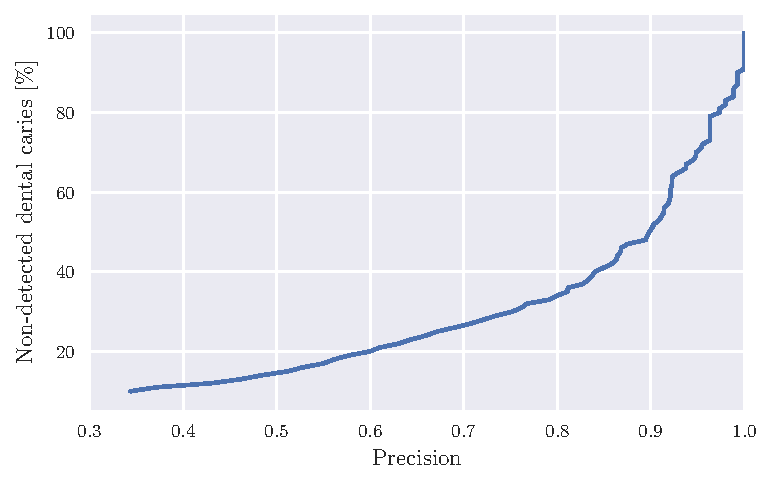
\includegraphics[width=\linewidth]{images/nondet_precision.pdf} }
    \end{floatrow}
\end{figure}

\begin{figure}[h]
    \centering
    \begin{subfigure}[b]{0.8\textwidth}
        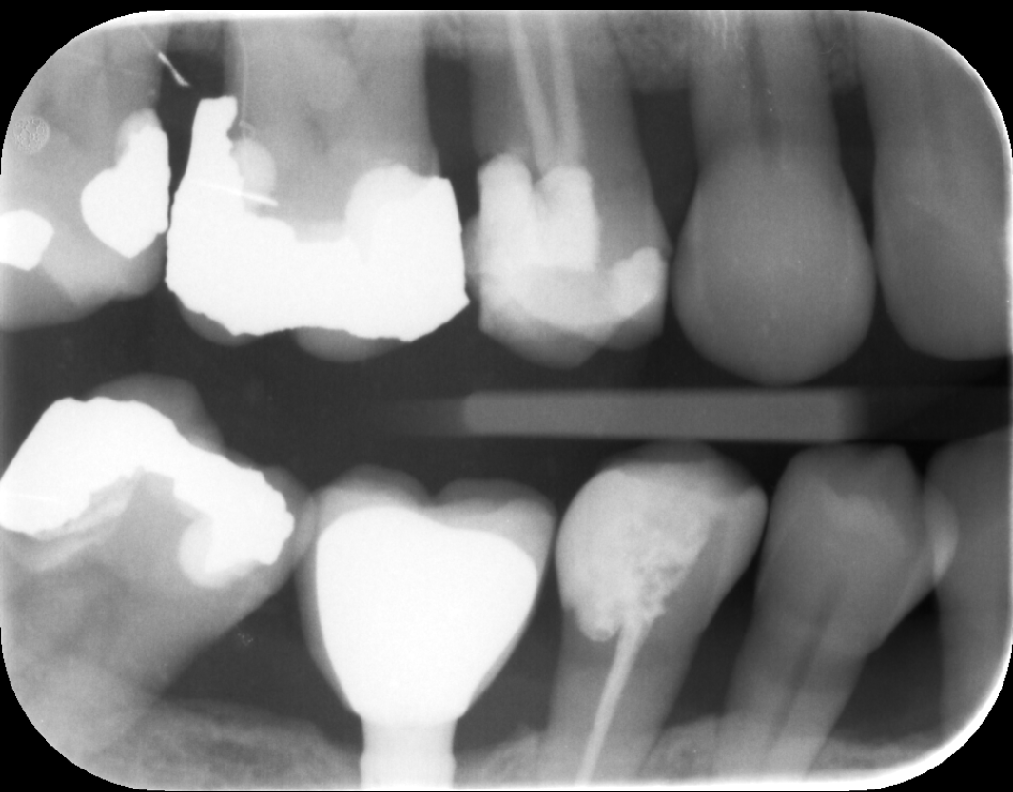
\includegraphics[width=1\linewidth]{images/det2orig.png}
        \caption{Original image}
    \end{subfigure}
    \begin{subfigure}[b]{0.8\textwidth}
        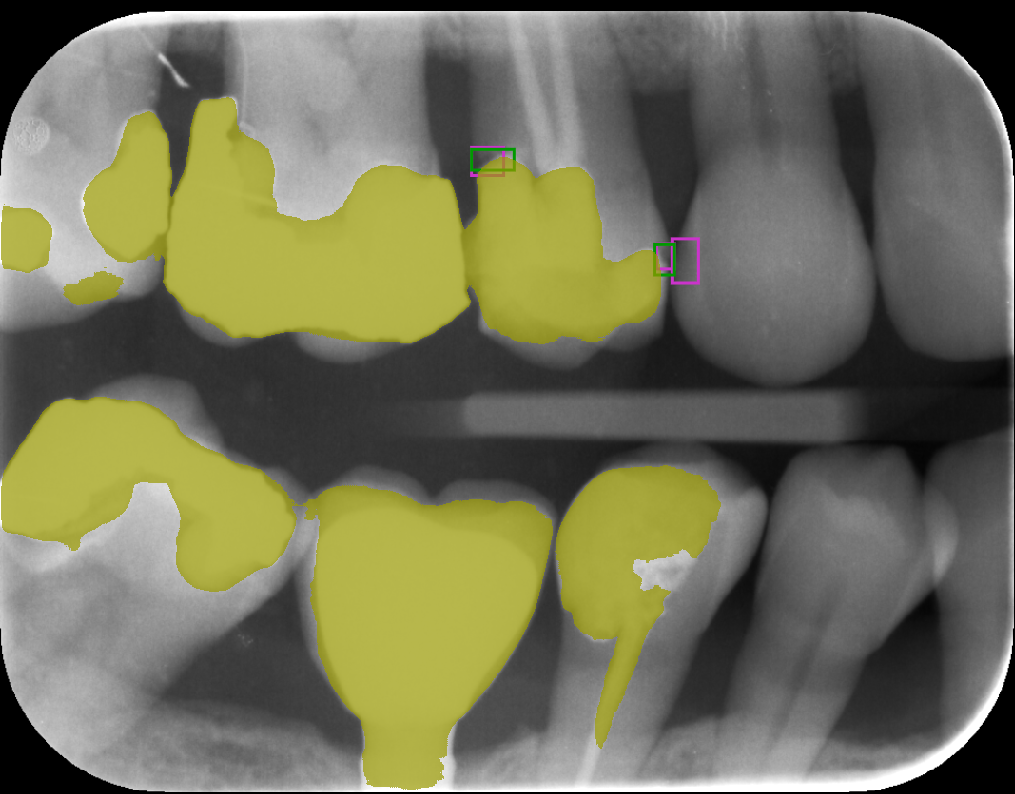
\includegraphics[width=1\linewidth]{images/det2pred.png}
        The o\caption{Output of our models}
    \end{subfigure}
    \caption{Segmented dental restorations in yellow, predicted dental caries in pink and ground truth of dental caries in green. We see a single false positive detection on the top right of the image. The author of the dataset acknowledges it to be a missing ground truth label}.
    \label{fig:both_models_1}
\end{figure}
